\section{Courseware}
\label{rasim:courseware}
%\todo{Introducir esto como contribución}
Todos los elementos anteriormente citados conforman un simulador de \ac{RV} por si mismo, pero no conforman una herramienta de entrenamiento sin un software que oriente al usuario en el proceso de aprendizaje. Por tanto, se ha contribuido en la creación del módulo \ac{Courseware}, que gestiona todos los componentes del simulador y se encarga de implementar todas las tareas de relacionadas con el entrenamiento. El software se ha diseñado con la finalidad de ser la interfaz del motor de \ac{RV} y ayude al usuario a interaccionar con él. Esto consigue que el simulador se convierta en una herramienta de aprendizaje y evaluación. Además, con el objetivo de garantizar un aprendizaje autónomo, este módulo deberá proporcionar una evaluación formativa y sumativa.  De esta forma, el \ac{Courseware} es el encargado de permitir al usuario identificarse y comunicarse con el servidor. En el servidor se almacenan los materiales multimedia y los escenarios que se cargarán en el simulador. La aplicación también es la encargada de inicializar el motor de \ac{RV} con los módulos de simulación. También es el encargado de presentar la interfaz gráfica que se mostrará a través de los monitores. Por una parte, mostrará la vista de paciente, y por otra la vista del \ac{Courseware}. Esta ventana contendrá a su vez la información del simulador de ultrasonidos y todos los botones y la información adicional asociada al modo de simulación que se esté ejecutando.

Este software permitirá comprobar si la herramienta de generación de \ac{VPH}, y por tanto la herramienta \ac{TPTVPH}, es útil para entrenar el procedimiento de \ac{RA}.



\subsection{Caso de uso}
\label{course:casodeuso}
El simulador estará emplazado en un centro de entrenamiento de profesionales de anestesia como una universidad o un hospital. Los usuarios utilizan el simulador con el objetivo de mejorar sus habilidades en el contexto de \ac{RA} y se pueden dividir entre estudiantes y profesionales. Los primeros utilizarán la herramienta para empezar su formación en \ac{RA}. Para los usuarios con conocimientos del procedimiento, la herramienta les ayudará a mejorar sus habilidades no cognitivas. Incluso, se espera que lo utilicen aquellos profesionales que están interesados en volver a practicar el procedimiento debido a que llevan tiempo apartados de su práctica.


El objetivo principal de la aplicación es la práctica de \ac{RA} en simulador orientado a dos perfiles de profesionales sanitarios.
\begin{itemize}
    \item \textbf{Estudiantes noveles:} Como herramienta de aprendizaje, la aplicación está orientado a introducir el procedimiento a nuevos anestesistas. Por tanto, es necesario que el entrenamiento sea inicialmente guiado, ofreciendo información adicional a lo largo del procedimiento. Será necesario un modo guiado que ayude al estudiante en el procedimiento de \ac{RA} paso por paso y pueda ofrecer ayuda si el usuario la requiere. El objetivo es que el usuario pueda mejorar sus habilidades cognitivas como las no cognitivas. Adicionalmente, el software recabará medidas de desempeño para que posteriormente puedan formar parte de una evaluación. Al final de la sesión, el sistema podrá mostrar los registros obtenidos sirviendo como evaluación formativa.

\item \textbf{Profesionales con conocimientos previos:} El simulador puede ayudar a sanitarios que quieran practicar o mejorar sus habilidades no-cognitivas. Como estos usuarios pueden tener conocimientos previos de \ac{RA}, se les permitirá saltarse el modo guiado ofreciéndole un modo sin restricciones. En este modo el usuario podrá actuar de manera libre mientras que el sistema registrará su rendimiento. Este podrá ser mostrado al final de la sesión que al igual que el modo guiado se podrá usar como evaluación formativa para el usuario.

\end{itemize}


Esta aplicación está diseñada para adaptarse al perfil del usuario. De este modo, la aplicación permite tanto un modo guiado y otro modo libre según el interés del usuario. 
Con el objetivo de fomentar el aprendizaje independiente, en sus primeros pasos la aplicación muestra material multimedia para facilitar la adaptación al simulador tanto para profesionales noveles como experimentados en \ac{RA}. En la herramienta se puede encontrar vídeos y ejemplos que muestran el funcionamiento de los elementos del simulador, así como material didáctico que abarca contenidos específicos del procedimiento de \ac{RA}.



\subsection{Requisitos}
\label{course:req}
A continuación, se detallarán los requisitos que vienen dados por el proyecto \ac{RASimAs} referentes al prototipo del simulador:


\begin{enumerate}
    \item Los usuarios adquirirán y desarrollarán las habilidades necesarias para realizar el procedimiento simulado que consiste en bloquear un nervio guiado por ultrasonidos, objetivo principal del procedimiento de \ac{RA}.
\item Anestesistas que hayan pasado tiempo sin realizar el procedimiento, podrán utilizar el simulador como método de reciclaje. Podrán practicar en el simulador antes de realizar el procedimiento en un entorno real. 
\item El simulador replicará los principales pasos del procedimiento.
\item El sistema identificará al usuario. Los estudiantes deberán introducir sus credenciales para que la aplicación recupere su información asociada del servidor.
\item  El sistema almacenará métricas de evaluación durante el uso del simulador y se las comunicará al servidor.
\item  La aplicación fomentará el aprendizaje independiente, sin necesidad de un supervisor durante el uso del simulador. El objetivo es mejorar el proceso de aprendizaje proporcionando ayuda antes, durante y después de la utilización del simulador. 

\item El usuario tendrá en todo momento disponible material multimedia que ayude a comenzar las sesiones de entrenamiento. Este material contendrá información útil tanto de aspectos específicos de \ac{RA} como de elementos del simulador.
\item Durante la sesión, la aplicación ofrecerá ayuda al usuario si se requiere. Descripción detallada de la tarea, ayuda para conseguir determinados objetivos, advertencias y errores.
\item Después de la sesión, el sistema podrá facilitar una retroalimentación al usuario.
\item Esta aplicación contará con funcionalidades adicionales con la finalidad de ayudar en la realización de la evaluación clínica del sistema.
\end{enumerate}





\subsection{Arquitectura}
\label{course:arq}
La arquitectura de la aplicación se ha diseñado de la siguiente manera (ver Fig. \ref{fig:coursearq}):
\begin{itemize}
    \item \ac{Courseware}: el módulo principal se encarga de arrancar los módulos de simulación, guía al usuario en el proceso, recoge las métricas e incluso implementa un sistema de reconocimiento de voz
\item Interfaz: este módulo se centra en manejar las ventanas que se mostrarán al usuario. Se encarga de los menús iniciales para acceder al sistema o navegar a través del material multimedia, muestra la interfaz en las sesiones de simulación y también muestra el resumen de la sesión al usuario.
\item Sistema comunicación: este módulo se encarga de las comunicaciones con el servidor para recuperar o actualizar el perfil del usuario.
\end{itemize}

\begin{figure}[h]
    \centering
    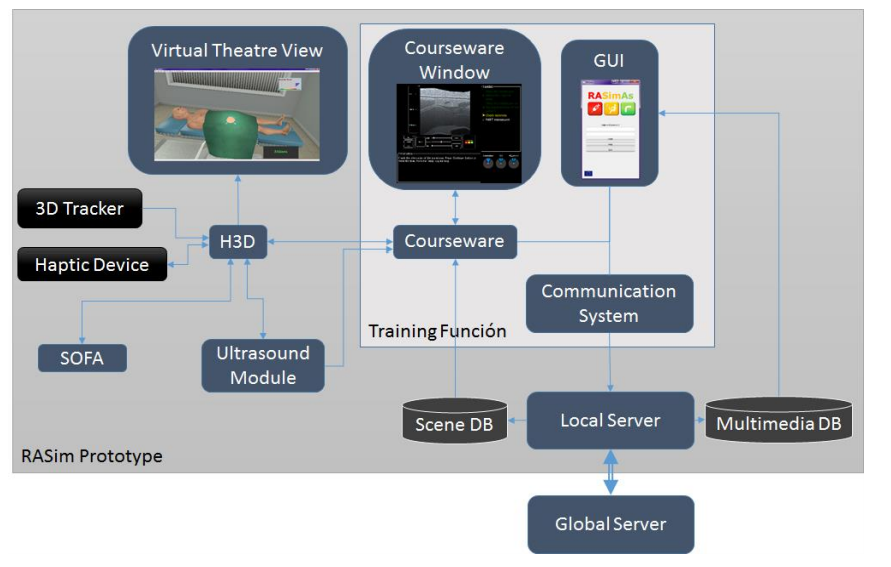
\includegraphics[width=0.5\textwidth]{IMG/coursewarearq.PNG}
    \caption{Diagrama inicial de la arquitectura de \ac{RASim}.}
    \label{fig:coursearq}
\end{figure}
\todo{rehago la imagen supongo}

Estos componentes del \ac{Courseware} se comunican con ciertos módulos externos del simulador:

\begin{itemize}
    \item \textbf{\ac{SOFA}}: El \ac{Courseware} es el encargado de seleccionar y especificar la escena que utilizará el módulo de simulación física. Así, se podrán recuperar métricas y variar parámetros de la simulación
    \item \textbf{\emph{H3D}}: También se comunicará con la simulación visual, con el objetivo de modificar y añadir ayudas visuales al usuario que se incorporarán en el modo guiado.
\item \textbf{\ac{US}}: El \ac{Courseware} está en todo momento comunicado con la simulación de \ac{US} para recuperar la imagen a mostrar, además de recuperar información adicional para la evaluación del sistema.


\item Servidor de RASim: El proyecto \ac{RASimAs} contempla la creación de un servidor que se usará para almacenar las escenas, modelos anatómicos, material multimedia y el perfil de los usuarios. Con el objetivo de no necesitar estar conectado a internet permanentemente, se ha diseñado un servidor local y otro global. El servidor local será instalado en el simulador de tal forma que periódicamente consulte nuevas actualizaciones o mande información al servidor global que comparten todos los simuladores.


\end{itemize}

Durante la simulación, el \ac{Courseware} interacciona con todos los módulos del núcleo de simulación. 
Aunque en los diseños originales del proyecto, las comunicaciones al módulo de \ac{US} se realizaban a través de la herramienta \emph{H3D}, debido a limitaciones de rendimiento, se decidió que el \ac{Courseware} fuera el centro de las comunicaciones. De esta manera, la información del simulador de \ac{US} es recibida directamente para utilizarla en la aplicación de entrenamiento. 

Por ejemplo, con el módulo de simulación física en ocasiones, como pueden ser el principio del procedimiento o fases de explicación, el \ac{Courseware} deshabilita ciertas comprobaciones que posibilitan al usuario adecuarse a los instrumentos. Así pues, hasta que el usuario no decide empezar con el ejercicio, no se recibe ninguna respuesta física por parte del dispositivo. 

Otro ejemplo de interacción con los módulos es la inclusión de ayudas visuales que se incorporarán a la simulación visual. Zonas iluminadas o figuras geométricas que ayudarán al usuario a entender los conceptos y pasos que deberá cumplir para finalizar el procedimiento. 



\subsection{Modos de simulación}
\label{course:modos}
Uno de los objetivos del \ac{Courseware} es el entrenamiento del procedimiento de \ac{RA} adaptándose al perfil del usuario. La aplicación proporciona dos modos de sesiones para adaptar la simulación a las necesidades del usuario. Los modos de simulación se definirán a continuación.

\subsubsection{Modo guiado}

El modo guiado está diseñado para adquirir habilidades cognitivas como no cognitivas. Está pensado para usuarios con poco conocimiento del procedimiento. Además, también puede servir para anestesistas que no haya practicar el procedimiento por un tiempo y necesita familiarizarse con el simulador antes de utilizar el modo libre. Parece evidente que usuarios con experiencia en \ac{RA} necesiten algunas sesiones guiadas para sentirse cómodos en la utilización del simulador. 
El modo guiado está diseñado para dirigir a los usuarios a través del procedimiento. El usuario será dirigido a través de pasos consecutivos hasta finalizar el procedimiento completo, estando limitado a realizar la tarea que se le indica. El modo guiado mostrará continuamente retroalimentación durante la sesión con el objetivo de ayudar al usuario  y se almacenarán métricas de evaluación que serán actualizadas en el perfil del usuario y mostradas al final de la sesión.

\todo{pongo aquí las ayudas o en UI?}

\subsubsection{Modo libre}

En el modo libre, el usuario puede realizar el procedimiento sin ninguna restricción y sin ninguna ayuda auxiliar por parte del \ac{Courseware}. Este modo esta orientado a que los usuarios puedan practicar sus habilidades no cognitivas en el procedimiento de \ac{RA}. La interfaz de usuario mostrada por la aplicación  y las métricas recogidas serán diferente que el modo guiado. Este modo no proporcionará ninguna información de apoyo y está orientada a recoger únicamente métricas del rendimiento del usuario en la sesión. Registrar estos parámetros presenta una dificultad extra ya que el usuario no está restringido como en el modo anterior, por lo cual la aplicación no conoce exactamente las intenciones del usuario. Aún así, se recogerán las métricas de elementos críticos del procedimiento como la inserción de la aguja.

En ambos modos de simulación, al finalizar la sesión, el usuario podrá observar las métricas recogidas por el simulador además de una información asociada a la métrica recogida. Estas métricas servirán como evaluación formativa.

\subsection{Interfaz de usuario}
\label{course:ui}
El \ac{Courseware} como responsable de supervisar a los otros módulos de simulación, se encargará de mostrar a los usuarios las ventanas con las que va a interaccionar. En la figura \ref{fig:simui} se puede observar las imagenes que se \emph{renderizarán} en cada monitor. En la imagen de la izquierda se puede observar la vista de paciente donde se puede apreciar la sala de operaciones virtual generada por el software \emph{H3D}. En la imagen de la derecha, se puede observar la interfaz del \ac{Courseware} cuando la simulación ya ha empezado. En ella se puede observar la imagen de \ac{US} acompañados de elementos que proporcionan información al usuario. A continuación, se describirán las interfaces por separado.

\begin{figure}[h]
    \centering
    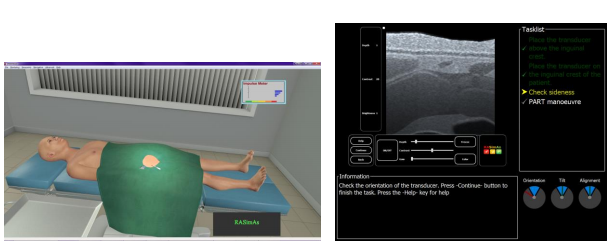
\includegraphics[width=0.5\textwidth]{IMG/simulatorui.PNG}
    \caption{Visualización de los dos monitores del simulador. A la izquierda se mostrará la vista de paciente, y a la derecha la interfaz del \ac{Courseware}.}
    \label{fig:simui}
\end{figure}

\subsubsection{Menús}

El primer contacto que tiene el usuario con el \ac{Courseware} es los menús asociados con la inicialización del sistema. En la figura \ref{fig:courseintro} se puede observar las interfaces que se encontrará el usuario al iniciar el programa. El primer paso es la identificación del usuario que será validado en el servidor. A continuación, se presenta el menú donde podrá elegir revisar el material multimedia como tutorial o seleccionar empezar la sesión en el modo guiado o libre. En el menú de tutorial podrá revisar el contenido multimedia que se encuentre en el simulador.

\begin{figure}[h]
    \centering
    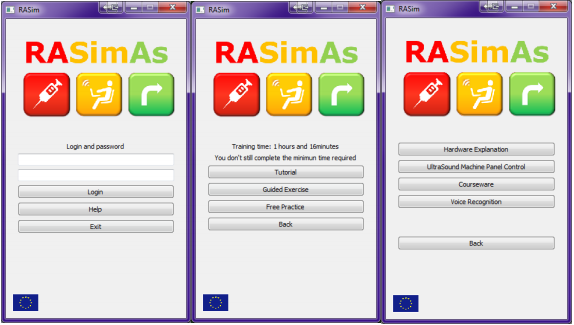
\includegraphics[width=0.5\textwidth]{IMG/coursewareintro.PNG}
    \caption{Menús contextuales. El usuario debe identificarse en el primero. En el segundo podrá elegir entre el tutorial y los modos de simulación, y en el último podrá visualizar el contenido multimedia disponible.}
    \label{fig:courseintro}
\end{figure}

\subsubsection{Modo guiado}

Como la finalidad de los dos modos de simulación son diferentes, las interfaces que presenta la aplicación son diferentes, debido a que en el modo guiado se proporciona información al usuario mientras que en el modo libre no existen ningún tipo de ayuda.

El modo guiado está orientado para guiar al usuario a lo largo del procedimiento de \ac{RA}. Por tanto, además de mostrar la información de \ac{US}, tiene que mostrar información adicional sobre la tarea actual, una lista de tareas, y dar la posibilidad de ofrecer ayuda al usuario. En la figura \ref{fig:guidedui}, se muestra un ejemplo de interfaz en una sesión guiada.
\begin{figure}[h]
    \centering
    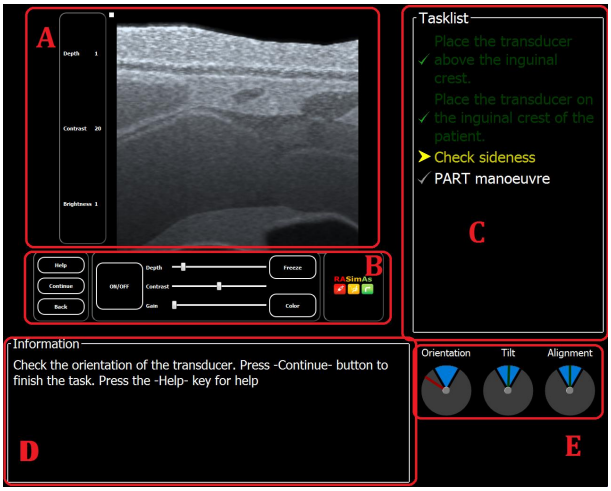
\includegraphics[width=0.5\textwidth]{IMG/guidedui.PNG}
    \caption{Instantánea de la interfaz del modo guiado}
    \label{fig:guidedui}
\end{figure}

\begin{itemize}
    \item En la división A y B se ha diseñado una interfaz lo más parecido a la máquina de \ac{US} \emph{Philips Sparq}\cite{Philips} (ver figura \ref{fig:philips}). En la división A se puede ver la imagen de \ac{US} con los parámetros actuales. En la división B se pueden ver el panel de control para configurar el \ac{US} y unas funcionalidades adicionales que se detallarán a continuación:
    \begin{enumerate}
        
        \item Botón \emph{On/Off}: apaga y enciende el simulador de \ac{US}.
        \item Botón \emph{Freeze}: congela la imagen de \ac{US}.
 \item Botón \emph{Color}: activa la tecnología de color \emph{Doppler} que se describirá en la sección \ref{doppler}.
\item Controles deslizantes: Permiten configurar la profundidad, el contraste y la ganancia del simulador de \ac{US}.
        \item Botón \emph{Help}: permite al usuario solicitar ayuda.
        \item Botones \emph{Continue y Back}: estos botones para permiten avanzar y retroceder en el procedimiento. 
    \end{enumerate}
    \item La lista de tareas del procedimiento de \ac{RA} se muestra en C.
    \item El panel D sirve para mostrar texto informativo sobre la tarea actual, mensajes de error o ayuda textual que requiera el usuario.
    \item Por último, en la división \emph{E} se muestran diferentes ayudas específicas de cada tarea.
\end{itemize}




\begin{figure}[h]
    \centering
    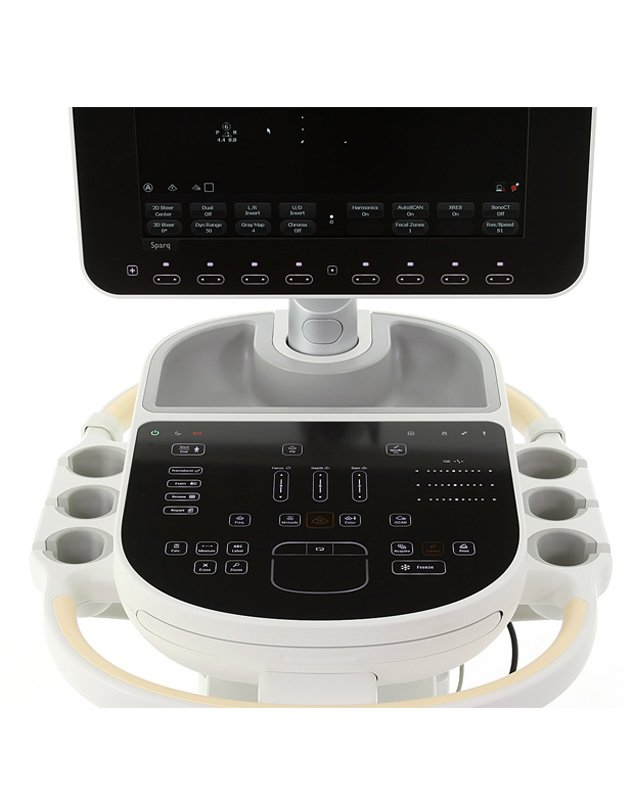
\includegraphics[width=0.5\textwidth]{IMG/philips.jpg}
    \caption{Máquina de \ac{US} \emph{Philips Sparq}\cite{Philips}}
    \label{fig:philips}
\end{figure}

\subsubsection{Modo libre}

En este modo, el sistema no debe presentar ninguna información de apoyo al usuario. Por tanto, la interfaz del \ac{Courseware} estará solo encargada de mostrar la imagen de \ac{US} y su panel de control como se puede observar en la figura \ref{fig:freeui}.

\begin{figure}[h]
    \centering
    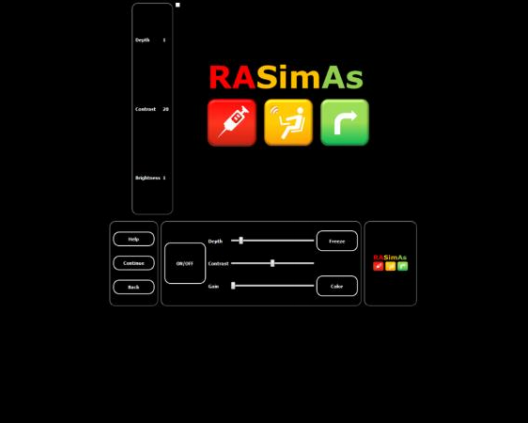
\includegraphics[width=0.5\textwidth]{IMG/freeui.PNG}
    \caption{Instantánea de la interfaz del modo libre}
    \label{fig:freeui}
\end{figure}


 

\subsection{Ayudas al usuario}
\label{course:ayudas}
El usuario puede solicitar ayuda mientras realiza la sesión guiada del procedimiento. Esta ayuda depende en gran medida de la tarea concreta que se este realizando en ese momento. Cada tarea tiene asociado una ayuda concreta ya que las tareas del procedimiento pueden ser muy diferentes entre sí. Si la ayuda que requiere el usuario es conceptual, el sistema mostrará un vídeo que contenga una explicación de la tarea a realizar, o puede ser simplemente muestre un mensaje en el panel de información. Otro ejemplo es la consecución de una posición correcta de los instrumentos médicos, de esta forma el simulador podrá añadir información visual que se superpondrá en la vista de paciente, o pueden ser ayudas específicas que se mostrarán en la interfaz del \ac{Courseware}. Por último, en cuanto a la interpretación de la imagen de \ac{US}, el usuario puede solicitar ayuda y el sistema mostrará información adicional en la imagen. A continuación se detallan de forma pormenorizada.


\subsubsection{Vídeos y ayudas textuales}

Si el usuario no ha entendido o no se acuerda de la realización de una tarea específica, la aplicación puede mostrar un texto de ayuda o un vídeo si el concepto es más complejo. Los textos de ayuda serán mostrados en la división D de la interfaz del sistema (fig. \ref{fig:guidedui}). En el caso de los vídeos, la aplicación abrirá una nueva ventana donde el usuario podrá ver la reproducción de un vídeo, pedir su repetición o cerrarla (fig. \ref{fig:video}).

\begin{figure}[h]
    \centering
    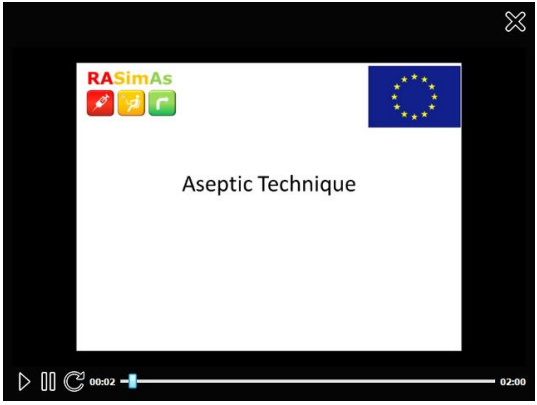
\includegraphics[width=0.5\textwidth]{IMG/video.PNG}
    \caption{Ventana para reproducir vídeos}
    \label{fig:video}
\end{figure}
 
\subsubsection{Ayudas visuales}

 En ocasiones, las ayudas son acerca de localizar alguna posición concreta fundamental en el procedimiento. Por ejemplo, el área de interés donde los instrumentos deben estar, o el punto de inserción de la aguja que se sitúa en una posición relativa a la sonda de \ac{US}. Estas ayudas se solicitan por el usuario y se podrán observar en la vista de paciente. En las figuras \ref{fig:viewhelp} y \ref{fig:viewhelp} se puede observar figuras geométricas transparentes que ayudan al usuario a localizarlas.
 
 
 \begin{figure}[h]
    \centering
    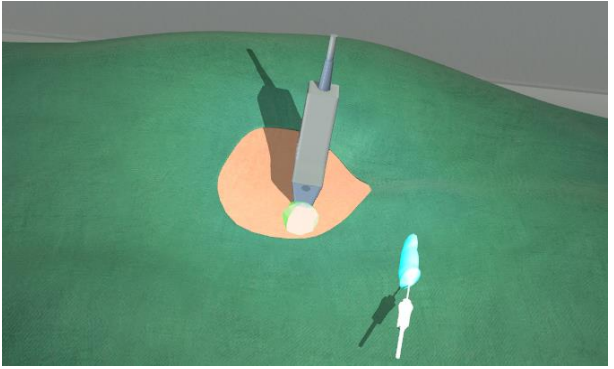
\includegraphics[width=0.5\textwidth]{IMG/viewhelp.PNG}
    \caption{Ayuda visual donde se puede observar una esfera que indica el punto de inserción de la aguja.}
    \label{fig:viewhelp}
\end{figure}

\todo{me falta otra imagen del cilindro}

Otro ejemplo es las recomendaciones de la rotación, orientación e inclinación de la sonda de \ac{US} para una correcta identificación de las estructuras anatómicas necesarias en el procedimiento. En el ejemplo visto anteriormente (ver Fig. \ref{fig:guidedui}), el complemento se puede observar en la división E.


\subsubsection{Ayudas en las imágenes de ultrasonidos}
Una de las mayores dificultades del procedimiento de \ac{RA} es identificar correctamente las estructuras anatómicas que son fundamentales para la localización del nervio. Si el usuario no está seguro de que estructuras ve en la imagen de \ac{US}, el sistema puede proporcionarle cierta ayuda coloreando las estructuras que debería identificar (ver Fig. \ref{fig:labelus}), junto con un mensaje que clarifica estos colores. Esto ha sido posible gracias a que el módulo de simulación de \ac{US}, además de proporcionar la imagen simulada, viene acompañada de una imagen con todas las estructuras anatómicas etiquetadas, con lo cual es fácil corresponder las dos imágenes.

 
 \begin{figure}[h]
    \centering
    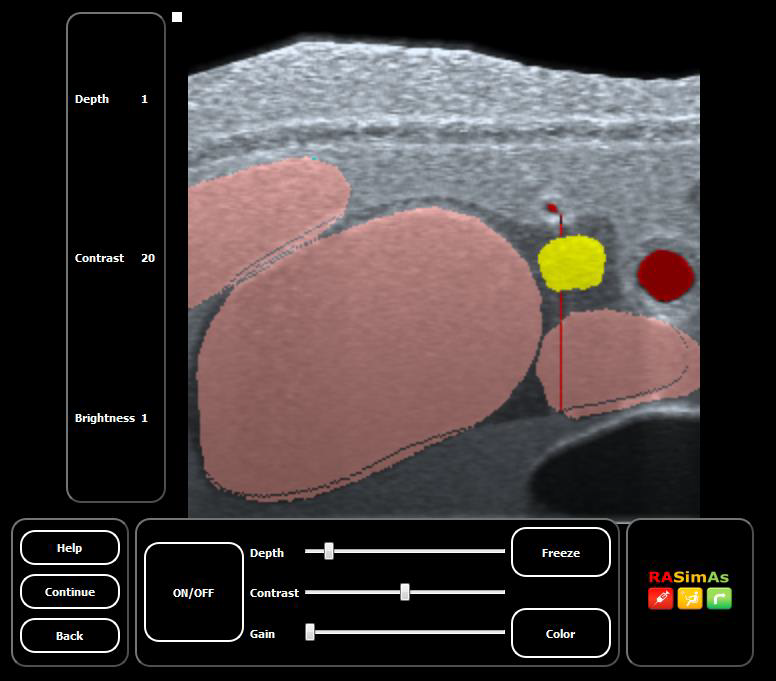
\includegraphics[width=0.5\textwidth]{IMG/labelus.png}
    \caption{Ayuda visual donde se puede observar ciertas estructuras anatómicas coloreadas. A la derecha se puede ver la imagen etiquetada correspondiente.}
    \label{fig:labelus}
\end{figure}
 
 
\subsubsection{Administración del anestésico}
 \begin{figure}[h]
    \centering
    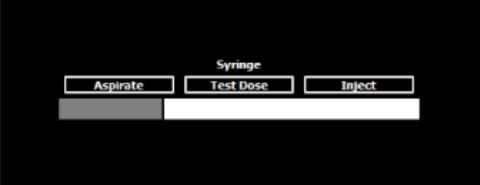
\includegraphics[width=0.5\textwidth]{IMG/Syringe.PNG}
    \caption{ Representación del contenido del anestésico en la jeringuilla y los botones asociados a su funcionalidad.}
    \label{fig:anest}
\end{figure}

Una de las partes fundamentales para saber si el procedimiento va a ser realizado satisfactoriamente es comprobar si la punta de la aguja se encuentra dentro de un vaso sanguíneo. El anestesista realiza una aspiración a través de la jeringuilla para comprobar que no haya sangre. A través de la interfaz de usuario del programa, se muestra una simulación de la jeringuilla con cierto contenido de anestésico como se puede observar en la figura \ref{fig:anest}. Esta interfaz servirá al usuario para saber si ha aspirado sangre o no, o cuanta cantidad de anestésico ha liberado para ejecutar la tarea de administrar una pequeña dosis. Aunque se han incluido unos botones para esta tarea, estas acciones pueden ser realizas a través del reconocedor de voz desarrollado para tal efecto, ya que los usuarios en esta etapa se encuentran con las manos ocupadas por los instrumentos médicos.




\subsubsection{Funcionalidad color \emph{Doppler}}
\label{doppler}
La funcionalidad color \emph{Doppler} es una técnica presente en los equipos de \ac{US} que consiste en mostrar velocidad, y dirección de un flujo sanguíneo superponiéndolo en la imagen de \ac{US}. Este efecto es muy fácil de simular al obtener toda la información desde el módulo de \ac{US}.
En la figura \ref{fig:doppler} se muestra la implementación de la funcionalidad color \emph{Doppler}.

\begin{figure}[h]
    \centering
    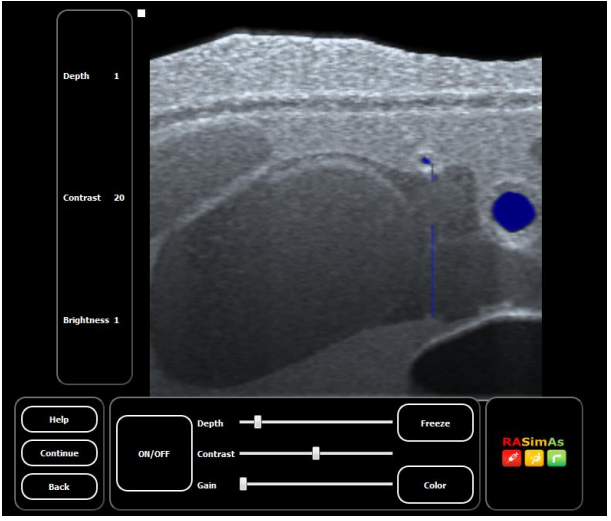
\includegraphics[width=0.5\textwidth]{IMG/uscolor.PNG}
    \caption{Demostración de la funcionalidad color Doppler}
    \label{fig:doppler}
\end{figure}


 
 
\subsubsection{Reconocimiento de voz}

El procedimiento de \ac{RA} no es un procedimiento que se realice exclusivamente por un anestesista. Lo habitual es que haya un asistente que  realice tareas secundarias dirigidas por la persona que está realizando el procedimiento. Esto es debido a que, en la mayor parte del tiempo del procedimiento, el médico tiene las manos ocupadas por la sonda de ultrasonidos y la aguja. Ciertas tareas, como administrar el anestésico, es realizado por el auxiliar mientras el anestesista supervisa el procedimiento. Aunque el simulador está orientado a que sea utilizado por una única persona y que las tareas no son complejas, se ha desarrollado un reconocimiento de voz para ejecutar ciertas tareas que permitirán al usuario realizar el procedimiento sin tener que soltar ninguno de los instrumentos. A continuación se definen los comandos diseñados para esta funcionalidad:

\begin{enumerate}
    \item \emph{Aspirate}: Antes de suministrar el anestésico, el médico debe comprobar si no se encuentra la punta de la aguja en un vaso sanguíneo. Para ello, retrae la inyección para comprobar que no haya sangre.
\item \emph{Release test dose}: Es habitual suministrar una pequeña dosis que haga al médico asegurarse de que va a suministrar en el sitio correcto y poderla localizarla en la imagen de \ac{US}.
\item \emph{Inject dose}: Administra el anestésico por completo.

\item Comandos auxiliares en el mod guiado:
\begin{itemize}
    \item \emph{I need help}: El usuario puede pedir ayuda para la tarea actual.
\item \emph{Option [one|two|three]}: El usuario selecciona una opción del menú contextual.

\end{itemize}

\end{enumerate}

 



\subsection{Retroalimentación final}
\label{course:feedback}
La evaluación formativa es un proceso en el que se realimenta el aprendizaje que posibilita su regulación directamente por el estudiante.\todo{revisar} De esta manera, junto con su supervisor, se puede inferir donde es necesario mejorar o incidir en determinadas actividades en relación con los resultados obtenidos. Con este objetivo, el simulador ofrece sesiones que hacen que el usuario pueda reforzar sus conocimientos y al finalizar el procedimiento, puedan observar el desempeño obtenido o los errores cometidos y actuar en consecuencia. Por ello, simuladores de \ac{RV} son utilizados con frecuencia con este motivo, ya que son capaces de registrar estas métricas de manera objetiva sin necesidad de la presencia de un supervisor. En el caso del simulador \ac{RASim} al final de cada sesión, el \ac{Courseware} muestra una ventana con las métricas obtenidas por el usuario. Estas métricas estarán coloreadas en verde si están dentro de un rango aceptable y en rojo si se han cometido errores o el valor a sobrepasado un límite. En la figura \ref{fig:resultui}, se puede observar un ejemplo de la ventana de resultados, donde se puede observar que las métricas se agrupan en tareas del procedimiento de \ac{RA}.



\begin{figure}[h]
    \centering
    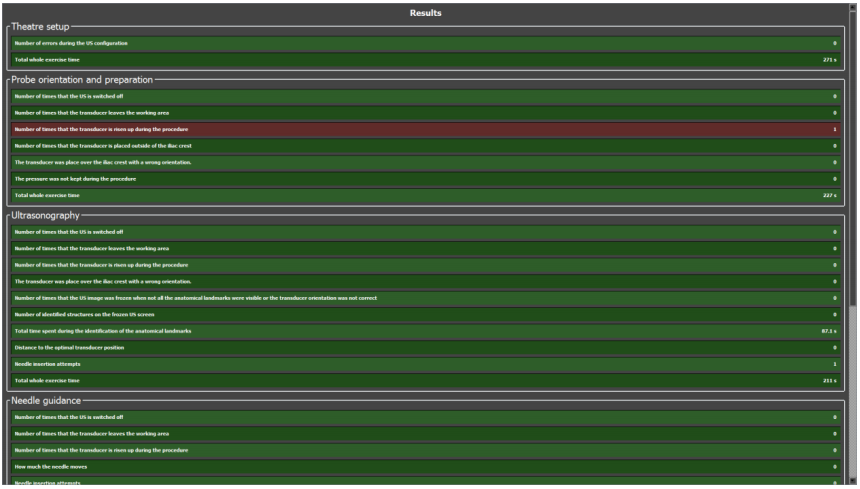
\includegraphics[width=0.5\textwidth]{IMG/resultui.PNG}
    \caption{Ventana donde se resumen todas las métricas recogidas. Con la finalidad de una evaluación formativa, se utiliza el color verde y rojo para mostrar una valoración del resultado.}
    \label{fig:resultui}
\end{figure}


\subsection{Métricas de evaluación}
\label{course:metricas}
Una de las funcionalidades importantes del simulador es medir el desempeño del usuario mientras realiza la sesión para su posterior evaluación. El \ac{Courseware} es el encargado de recopilar toda la información posible a través de la comunicación con los módulos del núcleo de simulación. Estas métricas serán utilizadas para dar retroalimentación al usuario de manera que constituya en una evaluación formativa. Las métricas se pueden clasificar en los siguientes tipos:

\begin{itemize}
    \item Situaciones de potencial riesgo para el paciente: En general estas métricas están asociadas a realizar el procedimiento de manera incorrecta. Ejemplos como levantar la sonda de ultrasonidos mientras la aguja está en el interior del paciente, extracción de la aguja de forma precipitada o repetidas inserciones, orientaciones de los instrumentos incorrectas, falta de evidencia de estructuras anatómicas en la imagen de \ac{US}, u omisión de pasos. 
    
    \item Tiempos: Tiempo empleado por el usuario en completar tareas, pasos y la sesión completa. 
    
    \item Número de repeticiones: Se registra el número de intentos de un paso concreto, o las veces que el usuario pide ayuda. Cuantas veces el usuario a perdido la zona de interés o los instrumentos médicos hayan salido de su posición óptima.
\end{itemize}


\subsection{Simulación de la difusión de la dosis}
\label{course:dosis}
La confirmación de que el anestésico está en el lugar adecuado es fundamental para conocer si el procedimiento ha sido realizado satisfactoriamente. Sin una solución clara, se presentaron varias propuestas con el objetivo que el consorcio de \ac{RASimAs}.

La primera propuesta era una simulación física que pudiera simular el comportamiento de introducir un fluido en un tejido. El tejido tendría que reaccionar deformándose además de poderse observar en la imagen de \ac{US}. En la figura \ref{fig:spread} se puede observar una versión inicial de esta propuesta, realizada en \emph{SOFA} con el objetivo de poder incluirla en la simulación física. Se intentaba resolver la difusión del fluido como si fuera la difusión de calor, teniendo en cuenta solo el tejido en el que había sido introducido sin afectar a los demás.

Esta propuesta presentaba varias limitaciones. Por una parte, no era viable la comunicación directa con el módulo de \ac{US} y hacía compleja su integración. Por otra parte, el nivel de detalle y complejidad necesario daba lugar a que el rendimiento de la simulación física se resintiera y no pudiera ser posible una interacción realista.

\begin{figure}[h]
    \centering
    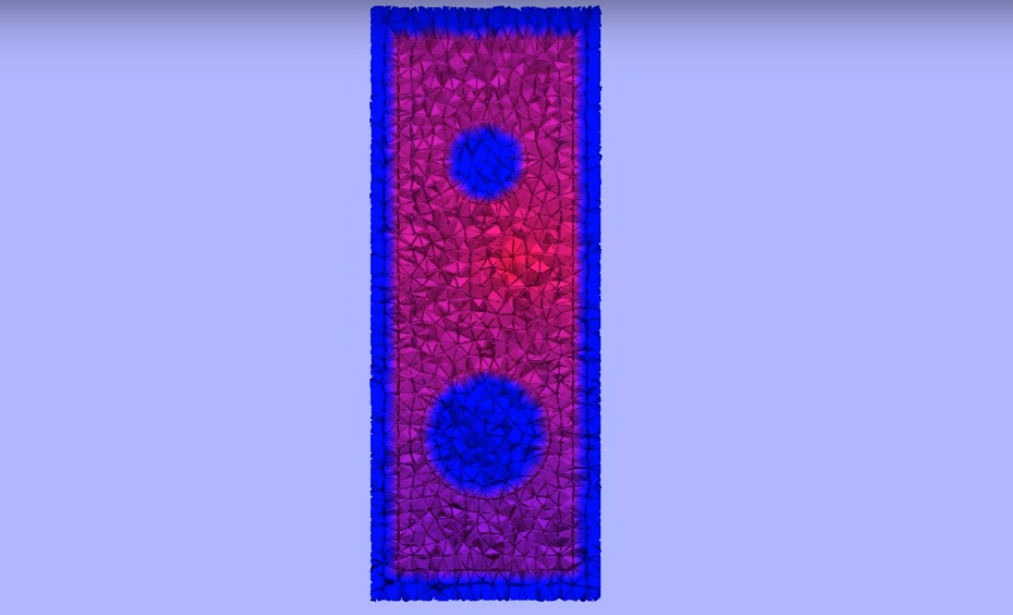
\includegraphics[width=0.5\textwidth]{IMG/spread.PNG}
    \caption{Simulación de difusión del anestésico utilizando la ecuación del calor. Los círculos representan otro tejido donde el fluido no afectaría.}
    \label{fig:spread}
\end{figure}

La segunda propuesta era una solución geométrica y heurística. Teniendo la imagen de \ac{US} segmentada y el tejido donde se encontraba la aguja, se le dio la responsabilidad al \ac{Courseware} de mostrar la difusión del fluido de forma geométrica únicamente en la imagen mostrada al usuario. En la figura \ref{fig:spread2} se puede observar como el anestésico es propagado virtualmente de forma esférica entre los tejidos donde fue insertado. Esta solución presenta el problema de que no deforma el tejido como si ocurre en la realidad.

\begin{figure}[h]
    \centering
    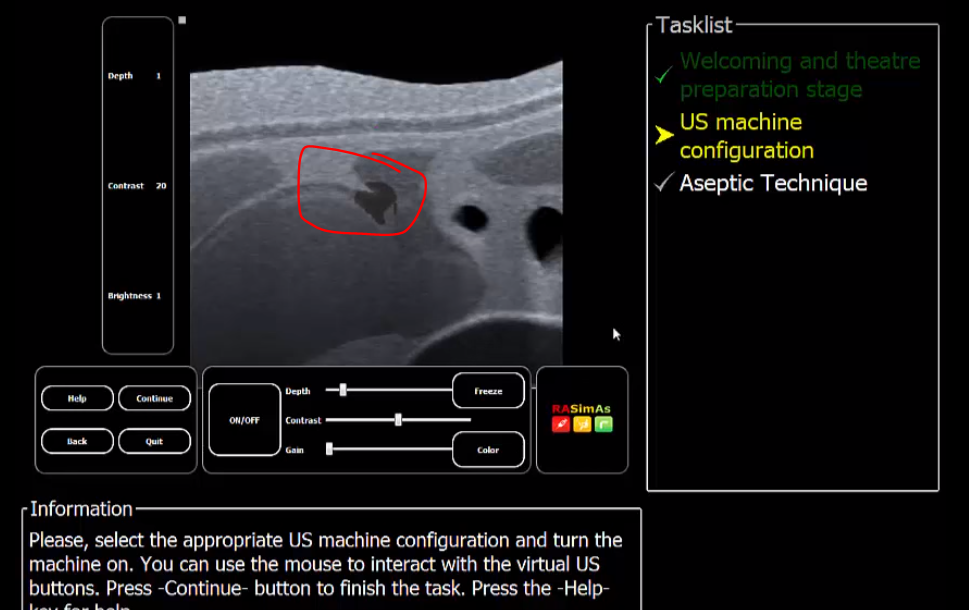
\includegraphics[width=0.5\textwidth]{IMG/spread2.PNG}
    \caption{Demostración de difusión esférica únicamente en la imagen de \ac{US}}
    \label{fig:spread2}
\end{figure}


% \subsubsection{External dependencies}
% During the Training Function implementation, some external APIs and standards
% have been used. All the employed external APIs can be used for free for prototyping
% and some of them have already been integrated in other RASimAs’ tasks.
% Additionally, since we decided to make our code portable, the external APIs are
% portable as well.
% The following list explains where the different APIs have been used:
% 1. JSON3
% is an international open standard format that uses human-readable text
% to transmit data objects consisting of attribute–value pairs. It is described by
% two competing standards RFC 7159 and ECMA-404. It has been used to
% communicate the server and the Training Function.
% 2. Qt4
% is a multi-platform library used to design UI widgets. It was used mainly to
% implement the UI. Additionally, Qt provides an abstraction layer, over JSON,
% which makes the communication with the server easier. Finally, this library
% was also used to implement the multimedia content player. It can be used
% under LGPL 2.1 or under a commercial license.
% 3. Qwt5
% is library that extends Qt with GUI components for technical applications.
% It has been employed to implant visual clues displayed on users demand. It
% can only be used under LGPL 2.1.
% 4. SimulationBase is a H3D6
% component that offers Python7 API to control the
% H3D simulation tree. It was used for detecting events on the virtual scene.
% 5. CMU Sphinx8
% is a speech recognition system. The Training System uses its
% module Pocketsphinx to implement the courseware’s voice recognition
% system. Pocketsphinx can be used under BSD.
% 6. ZeroMQ9


